\chapter{Conclusion}

\section{New Horizons for Biodiversity Monitoring}

It is not necessarily the case that access to more information on the state of biodiversity means that we will collectively make more informed choices about land use planning in favor of conservation. Dire and repeated warnings about the consequences of environmental change often appear unheeded, as local or national priorities—the scales at which all land management decisions are made—supersede global and ecological priorities \cite{Ehrlich1983-xx, Daily1999-mv, Barnosky2012-wi, IPBES2019-hl}. But information from monitoring efforts have led to dramatic changes in public policy in the past, like reducing the deforestation rate by 70\% in the Amazon following some of the first satellite-based land cover change analyses \cite{Roughgarden1991-so, Skole1993-jt, Nepstad2014-ar} and increasing reforestation in northwestern China following severe flooding and encroaching desertification \cite{Michael_A_Fullen1994-ip, Ye2005-vm}. Like independent journalism, biodiversity monitoring systems are a necessary but insufficient institution, informing public and official discourse on how human activities are changing global ecological processes and how these changes might be mitigated. Reporting this information clearly, credibly, and transparently will be especially important in the coming decade, as the greatest threat to conservation and climate change mitigation is likely to be the widespread transmission of bad-faith disinformation \cite{Iyengar2018-ij}.

Satellites and other earth observing sensors are essential monitoring tools, providing repeat, thematically consistent, and globally available measurements of the earth's ecosystems. But these abundant measurements are difficult to translate into metrics that are biological, subject to change, and ecosystem agnostic, limiting adoption according to current biodiversity monitoring protocols \cite{Geo_bon2017-ak}. This dissertation reviewed and addressed some of the technical and conceptual challenges to mapping biodiversity patterns from satellite imagery, including addressing scale gaps between satellite and \textit{in situ} data, using machine learning to simulate ecological processes, and handling biased or incomplete species data to characterize niche use patterns and predict spatial distributions. From these analyses emerges a flexible, scalable approach to measuring, monitoring and forecasting biodiversity change, highlighting opportunities to establish earth observations as the backbone of novel biodiversity monitoring systems. Three takeaways characterize the lessons learned from this work.

\begin{enumerate}
    \item Biodiversity mapping analyses should include multi-scale environmental covariate data when linking satellite and \textit{in situ} data. Local biodiversity patterns are often driven by ecological processes that operate at multiple spatial scales, and intermediate-scale patterns like disturbance regimes are often poorly represented in models that directly link fine-grained field data with coarse-grained environmental data. Multi-scale modeling approaches like \cite{Baccini2017-zk}, reviewed in detail in \textit{Chapter 2}, illustrate how integrating multiple data sources can translate biodiversity patterns from field to global scales, while characterizing the relative importance of multiple intersecting drivers of change.
    \item Models can precisely translate earth observations measurements from units of energy into units of biodiversity when model form and covariate transformations are tailored to a specific domain of scale. Spectral reflectance patterns have different underlying drivers at the leaf, canopy, and community scales, and \textit{Chapter 3} showed how isolating the drivers of canopy reflectance into discrete features dramatically improved species mapping accuracy, performing better than more complex neural network models trained with the same data \cite{Marconi2018-wn}.
    \item Biomimicry is a powerful approach to selecting and training machine learning algorithms to approximate and investigate ecological processes. While several processes can be characterized in lab environments, including temperature-dependent metabolic responses in ectotherms, many other processes like habitat use are harder to quantify in controlled settings. In \textit{Chapter 4} we trained models that mimicked the form of a known ecological process, nonlinear thermal response functions, to fit similar functions quantifying mosquito-habitat and mosquito-resource relationships, which revealed previously under-recognized drivers of the spatial distributions of two globally invasive arbovirus disease vectors.
\end{enumerate}

\noindent With more earth observations sensors slated to launch, access to biodiversity data increasing, and the development of new modeling approaches that integrate these data to produce globally-consistent metrics of biodiversity change, the promise of global biodiversity monitoring is becoming a reality. And it is not a moment too soon, with the effects of climate change and biodiversity loss already manifesting. How should we, collectively, use all of this new biodiversity information? And what purposes could monitoring systems serve if they were able to provide spatially and taxonomically complete information on the state of biodiversity?

\begin{figure}[!ht]
    \centering
    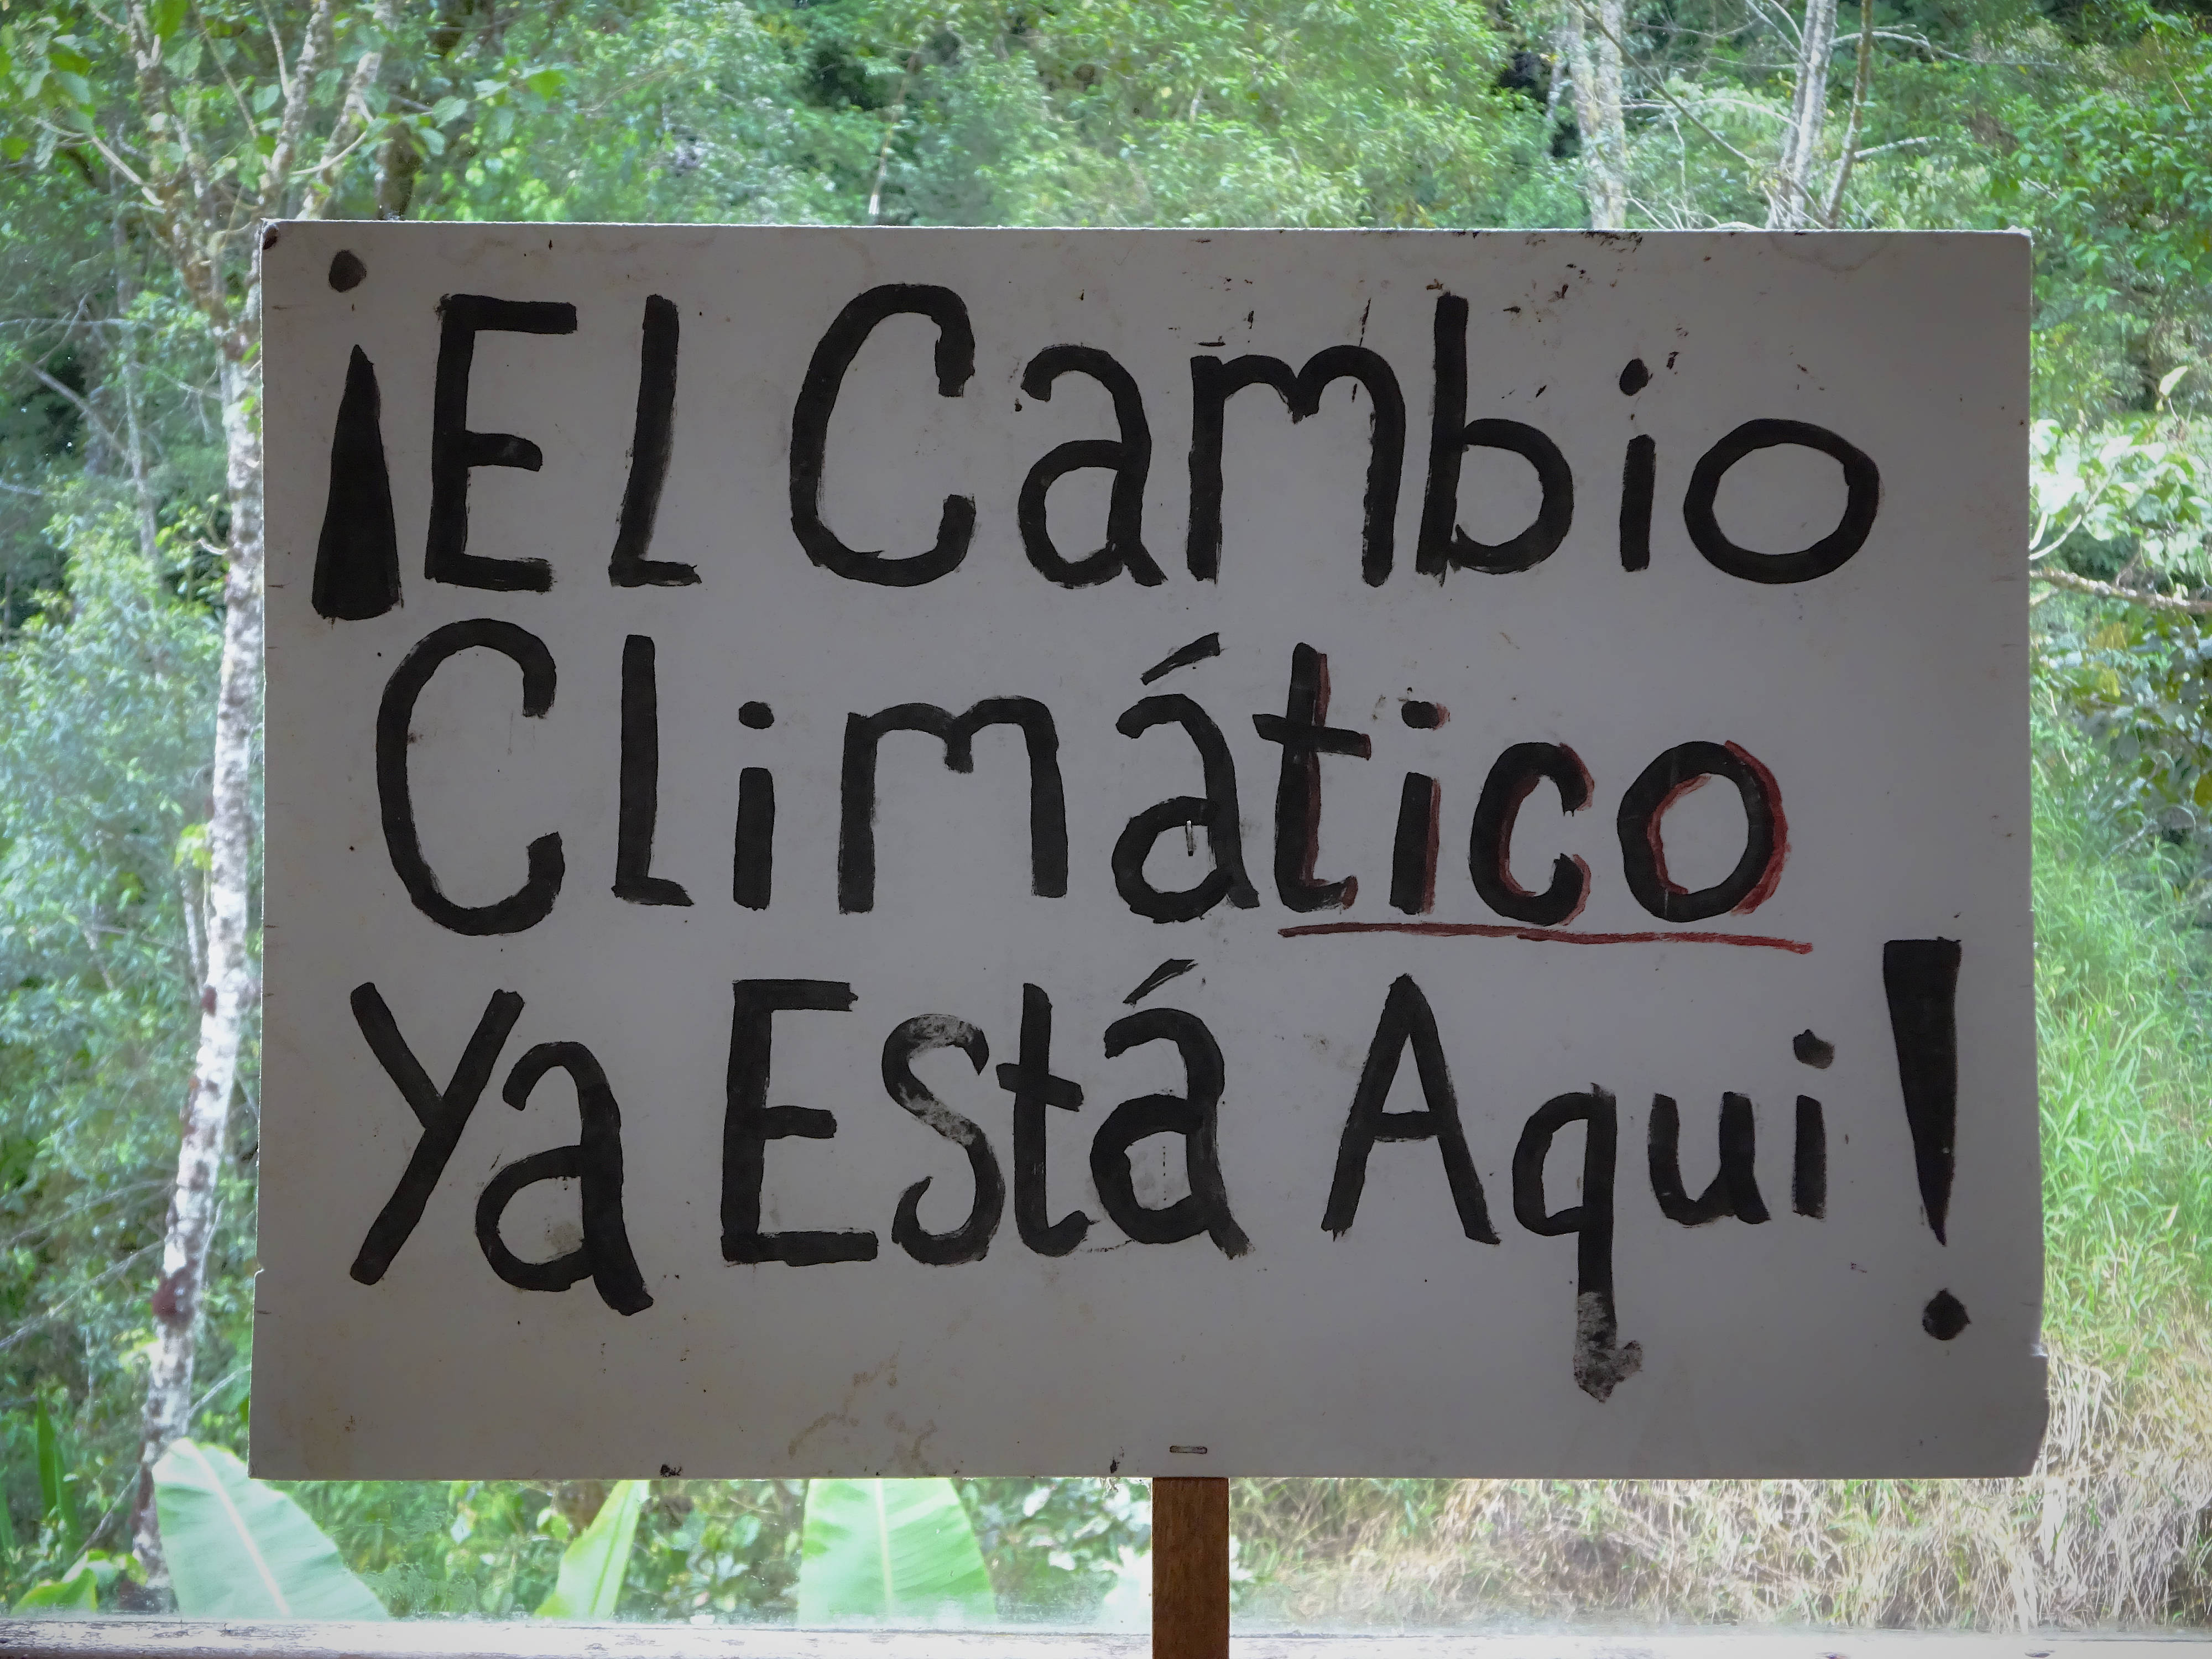
\includegraphics[width=\textwidth]{figures/conclusions-climate-change.jpg}
    \caption{A sign on Mount Chirripó in Costa Rica, home to the only high altitude Páramo grassland system in Mesoamerica, announcing that climate change has already arrived.}
    \label{fig:climage-change}
\end{figure}

\section{Acting on Complete Information}

If the central challenge addressed in this dissertation was how to translate earth observations measurements from units of energy into units of biodiversity, the challenge posed by the preceding questions regards how to translate complete biodiversity information into effective conservation action. To clarify, by discussing ``complete information" I'm encouraging a thought experiment regarding how we should use perfect knowledge of the state of the biosphere, and not suggesting that earth observations technologies alone will soon deliver this knowledge. This is certainly a topic too broad to address in much depth here. But as far as I can discern, there are four main opportunities for biodiversity monitoring systems to mitigate the risks posed by biodiversity change.

The first opportunity is to systematically quantify the conservation status of species, communities, and ecosystems to identify what is at risk, then design mitigation strategies. While this may seem a simplistic or obvious task—and already the central goal of existing international conservation treaties like the Convention on Biological Diversity's Aichi Biodiversity Targets—existing efforts to mitigate risks are still severely data limited. \cite{Geijzendorffer2016-xv} found that, while global commitments to halting biodiversity loss have been signed, requiring extensive monitoring and evaluation to take action, the data available to evaluate conservation status in accordance with their reporting standards covers less than 25\% of stated monitoring targets in some cases. This problem is especially acute for patterns of genetic diversity and ecosystem function, while data on trends in species populations are typically the most comprehensive. Incomplete information is a convenient and often legitimate excuse for inaction; complete information would remove this barrier.

The next opportunity is to analyze the historical satellite record and, based on the direction and magnitude of recent changes, design early-warning forecasts to predict upcoming threats to people and to species populations. As new data sharing policies have enabled open access to a long record of detailed satellite earth observations (Fig. \ref{fig:timeline}), new temporally-explicit methods have been developed to map change over time using process-based and machine learning models \cite{Cohen2018-xk, Rao2020-qk}, which could be used to forecast near-term ecological changes and guide investments in conservation and restoration. A similar approach is being deployed in China following their recent National Ecosystem Assessment, where the impacts of a decade of land use change following a \$50bn investment in environmental restoration and urbanization were used to guide a much larger investment in conservation in the coming years based on the trends that were declining \cite{Ouyang2016-il, Bryan2018-xz}.

These kinds of large-scale investments aimed at improving the sustainability of land management practices have dramatically increased from both private and public sources over the past decade \cite{hamrick2016state}. The monitoring, reporting, and verification standards associated with these investments are often inconsistently defined and applied, however, leaving many to wonder about the actual returns on these investments \cite{Ferraro2006-gj, Engel2008-bq, Sexton2016-vb}. With so much at stake, there is a lot of pressure on scientists to quantitatively measure and monitor the changes that occur as a result these investments, and this emerged as a top priority following the previously mentioned National Ecosystem Assessment [Z. Ouyang, pers. communication]. The good news is that a global synthesis found the rate of biodiversity loss decreased directly in response the amount invested in conservation \cite{Waldron2017-ct}. The bad news is that the effectiveness of this spending decreased as development pressures increased, and over one third of the areas protected since 1992 have experienced and increase in development pressure \cite{Jones2018-uv}. Quantifying biodiversity change simultaneously with the drivers of change—putting people on the map \cite{Ellis2008-xj}—is another key opportunity for monitoring systems.

The final opportunity, and the most urgent, is to increase public access to biodiversity information. Access—the ability to derive benefits from resources \cite{Ribot2009-wm}—to biodiversity itself is declining globally, due in part to increasing rates of urbanization \cite{United_Nations_Population_Division_undated-nr, Bratman2019-hi} as well as the large-scale transfer of land from small private landowners and governments to large companies, often through land grabs \cite{Peluso2011-rl, Borras2012-gr, Wolford2013-vh}. Access to biodiversity information, as well as the technical expertise required to analyze and understand it, is especially limited in poor communities in disadvantaged regions—the communities being excluded from accessing nature's benefits—which is also where the negative effects of biodiversity and climate change are expected to be most severe (Fig. \ref{fig:climage-change}) \cite{Borras2012-or, Richardson2016-lq, Barbier2018-nw, IPBES2019-hl}. It is imperative that information detailing biodiversity change and the human impacts of these changes, such as shifting exposure to vector-borne diseases, be made both accessible and useful to the populations that are most vulnerable.

Complete information on the state of biodiversity alone is insufficient for catalyzing large-scale conservation action, and the degree to which we will collectively use such information to create a more just and sustainable world will depend on the ability and willingness of monitoring institutions to make biodiversity information clear, credible, and transparent to the public. And with intergovernmental organizations ceding the responsibility of monitoring to national and regional bodies, electing instead to focus on capacity building and filling data gaps \cite{Larigauderie2010-rp, Scholes2012-ec}, perhaps there is an opportunity to build an independent global biodiversity monitoring institution based on these principles.